The \gls{descan} is an R \cite{Ihaka1996} tool developed for detecting epigenomic signal in order to facilitate the \glspl{der} between two or more biological conditions.

The package has been implemented using Bioconductor \cite{Gentleman2004} data structures and methods, and it is available on Bioconductor since version 3.7.

\begin{figure}[H]
\centering
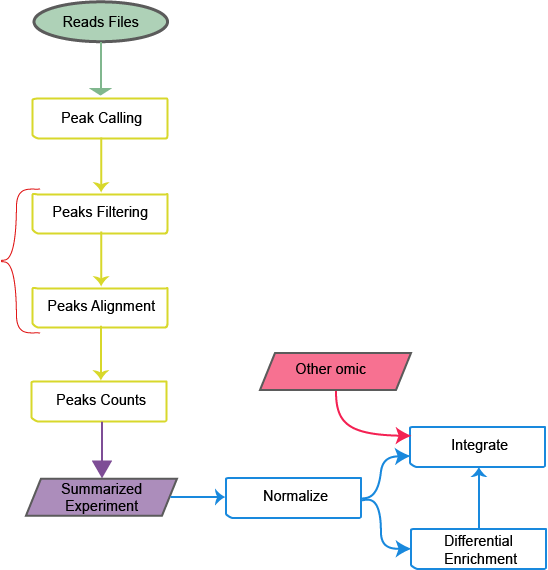
\includegraphics[width=\textwidth,height=\textheight,keepaspectratio]{img/descan2/flow.png}
\caption[DEScan2 workflow]{A differential enrichement flow representation. \gls{descan} steps are highlighed in yellow.}
\label{fig:descan2flow}
\end{figure}

The tool is organized in three main steps. 
A peak caller, which is a standard moving scan window that compares the counts within a sliding window, to the counts in a larger region outside the window. It uses a Maximum Likelihood Estimator on a Poisson Distribution, providing a final score for each detected peak.


The filtering step is aimed to determine if a peak is a "true peak" on the basis of its replicability in other samples. This step is based on a double user-defined threshold, one on the peak's scores and one on the number of samples.


Finally, the third step produces a counts matrix where each column represents a sample and each row a peak. The value of each cell is the number of reads for the peak in the sample.

The so produced counts matrix, as illustrated in the figure \ref{fig:descan2flow}, is useful both for doing differential enrichment between multiple conditions and for integrating the epigenomic data with other -omic data types.




